\chapter{曲线积分}

本章讨论第一类曲线积分和第二类曲线积分。

“第一类曲线积分”是数量值函数对曲线的积分,表示数量值对于一个曲线路径的累积量,和重积分的区别在于积分区域,除此之外没有任何区别。
“第二类曲线积分”是向量值函数对曲线的积分,是向量值在某个方向上的,具体说是在某点处的曲线方向的投影对曲线路径的累积量,与第一类曲线积分相比,多了一个“投影”步骤,表达式上是两个矢量的内积。

本章要点:
\begin{itemize}
    \item 第一类曲线积分。
    \item 第二类曲线积分。
\end{itemize}

~

\newpage
\section{第一类曲线积分}

本节讨论第一类曲线积分。
所谓“第一类曲线积分”是数量值函数对曲线的积分。

本节要点:
\begin{itemize}
    \item 掌握第一类曲线积分的概念;
    \item 掌握第一类曲线积分的计算,重点掌握弧微分的计算。
\end{itemize}

%============================================================
\subsection{第一类曲线积分的概念}

\begin{definition}[第一类曲线积分]
若三维空间中有曲线$L$,$f\left( \boldsymbol{p} \right) ,\boldsymbol{p}\in \mathbb{R} ^3$为定义在该空间上的三元数量值函数,若下式极限存在,则称极限值为{\bf $f\left( \boldsymbol{p} \right) $在$L$上积分称为第一类曲线积分},记为$\int_L{f\left( \boldsymbol{p} \right) dl}$,即:
\[
\int\limits_L{f\left( \boldsymbol{p} \right) dl}:=\underset{\lambda \rightarrow 0}{\lim}\sum_{i=1}^n{\left[ f\left( \xi _i,\eta _i,\zeta _i \right) \cdot \Delta l_i \right]}
\]
其中:
\begin{itemize}
    \item $f\left( \boldsymbol{p} \right) $:{\bf 被积函数};
    \item $dl$:{\bf 弧微分};
    \item $L$:{\bf 积分曲线}。
\end{itemize}
\end{definition}

\begin{tcolorbox}
实际定义参考“教材\cite{book1}”,这里是一个简写,总体来讲就是将曲线分段,每段上取一个值和这一小段弧长乘积$f\left( \xi _i,\eta _i,\zeta _i \right) \cdot \Delta l_i$,如果和式有极限,则称为$f\left( \boldsymbol{p} \right) $在$L$上有第一类曲线积分。
大致思路和一元函数积分一样。
\end{tcolorbox}

第一类曲线积分的性质:
\begin{itemize}
    \item 线性性:
    \[
    \int\limits_L{\left( af+bg \right) dl}=a\int\limits_L{fdl}+b\int\limits_L{gdl}
    \]
    \item 区域可加性:
    \[
    \int\limits_L{fdl}=\int\limits_{L_1}{fdl}+\int\limits_{L_2}{fdl}
    \]
\end{itemize}

同样,可定义$n$维空间上的数量值函数$f\left( \boldsymbol{p} \right) ,\boldsymbol{p}\in \mathbb{R} ^n$对空间内曲线$L$上积分为$f\left( \boldsymbol{p} \right) $在$n$维空间曲线$L$上的第一类曲线积分,记为$\int_L{f\left( \boldsymbol{p} \right) dl}$。

%============================================================
\subsection{第一类曲线积分的计算}

\begin{theorem}[第一类曲线积分的计算公式]
设三维空间上有曲线$L$,则曲线可以写为:
\[
L:\begin{cases}
	x=x\left( t \right)\\
	y=y\left( t \right)\\
	z=z\left( t \right)\\
\end{cases}
\]
弧微分的表达式:
\begin{align*}
dl&=\sqrt{\left( dx \right) ^2+\left( dy \right) ^2+\left( dz \right) ^2}=\sqrt{\left( x'dt \right) ^2+\left( y'dt \right) ^2+\left( z'dt \right) ^2} \\
&=\sqrt{\left( x' \right) ^2+\left( y' \right) ^2+\left( z' \right) ^2}\cdot dt
\end{align*}
若$f\left( \boldsymbol{p} \right) $在曲线$L$的$\left[ t_1,t_2 \right] $上连续,其中$x\left( t \right) ,y\left( t \right) ,z\left( t \right) $在$\left[ t_1,t_2 \right] $上具有一阶连续导数,则第一类曲线积分可计算为:
\[
\int\limits_L{f\left( \boldsymbol{p} \right) \cdot dl}=\int\limits_L{f\left( x,y,z \right) \cdot \sqrt{\left( x' \right) ^2+\left( y' \right) ^2+\left( z' \right) ^2}\cdot dt}
\]
\end{theorem}






\newpage
\section{第二类曲线积分}

本节讨论第二类曲线积分。
所谓“第二类曲线积分”是向量值函数对曲线的积分。

本节要点:
\begin{itemize}
    \item 掌握第二类曲线积分的概念;
    \item 掌握第二类曲线积分的计算,重点掌握积分表达式的内积计算。
\end{itemize}

%============================================================
\subsection{第二类曲线积分的概念}

\begin{definition}[第二类曲线积分]
若三维空间中有曲线$L$,$\mathbf{n}\left( \boldsymbol{p} \right) $为曲线上任一点处的单位切向量,$\boldsymbol{f}\left( \boldsymbol{p} \right) $为定义在该空间上的三元向量值函数,若内积$\boldsymbol{f}\left( \boldsymbol{p} \right) ^T\mathbf{n}\left( \boldsymbol{p} \right) $在$L$上的第一类曲线积分存在,则称此积分值为{\bf $\boldsymbol{f}\left( \boldsymbol{p} \right) $在$L$上的第二类曲线积分},记为$\int_L{\left[ \boldsymbol{f}\left( \boldsymbol{p} \right) ^T\mathbf{n}\left( \boldsymbol{p} \right) \right] \cdot dl}$,由于$\mathbf{n}\left( \boldsymbol{p} \right) dl=\boldsymbol{dl}$为弧微分在{\it xyz}坐标的投影向量,所以也可以写为$\int_L{\boldsymbol{f}\left( \boldsymbol{p} \right) ^T\boldsymbol{dl}}$,即:
\begin{align*}
&\int\limits_L{\left[ \boldsymbol{f}\left( \boldsymbol{p} \right) ^T\mathbf{n}\left( \boldsymbol{p} \right) \right] \cdot dl}=\int\limits_L{\boldsymbol{f}\left( \boldsymbol{p} \right) ^T\boldsymbol{dl}} \\
&:=\underset{\lambda \rightarrow 0}{\lim}\sum_{i=1}^n{\left[ \boldsymbol{f}\left( \xi _i,\eta _i,\zeta _i \right) ^T\mathbf{n}\left( \xi _i,\eta _i,\zeta _i \right) \cdot \Delta l_i \right]}
\end{align*}
其中:
\begin{itemize}
    \item $\boldsymbol{f}\left( \boldsymbol{p} \right) $:{\bf 被积函数};
    \item $\mathbf{n}\left( \boldsymbol{p} \right) $:曲线上任一点处的{\bf 单位切向量},也即切线的方向余弦;
    \item $\boldsymbol{dl}=\mathbf{n}\left( \boldsymbol{p} \right) dl$:{\bf 有向弧微分};
    \item $L,t\in \left[ t_1,t_2 \right] $:{\bf 积分曲线}。
\end{itemize}
特别地,当$L$为封闭曲线时,记为$\oint_L{\boldsymbol{f}\left( \boldsymbol{p} \right) ^T\boldsymbol{dl}}$。
\end{definition}

这里要注意,第二类曲线积分是有方向性的,$t_1\rightarrow t_2$的方向是切线的方向,如果取反方向,则写为:
\[
\int\limits_{L^-}{\boldsymbol{f}\left( \boldsymbol{p} \right) ^T\boldsymbol{dl}}
\]

第二类曲线积分的性质:
\begin{itemize}
    \item 线性性:
    \[
    \int\limits_L{\left( a\boldsymbol{f}+b\boldsymbol{g} \right) ^T\boldsymbol{dl}}=a\int\limits_L{\boldsymbol{f}^T\boldsymbol{dl}}+b\int\limits_L{\boldsymbol{g}^T\boldsymbol{dl}}
    \]
    \item 区域可加性:
    \[
    \int\limits_L{\boldsymbol{f}^T\boldsymbol{dl}}=\int\limits_{L_1}{\boldsymbol{f}^T\boldsymbol{dl}}+\int\limits_{L_2}{\boldsymbol{f}^T\boldsymbol{dl}}
    \]
    \item 有向性:
    \[
    \int\limits_{L^-}{\boldsymbol{f}^T\boldsymbol{dl}}=-\int\limits_L{\boldsymbol{f}^T\boldsymbol{dl}}
    \]
\end{itemize}

%============================================================
\subsection{第二类曲线积分的计算}

\begin{theorem}[第二类曲线积分的计算公式]
曲线在某点的切向量:
\[
\boldsymbol{n}\left( \boldsymbol{p}_0 \right) =\left. \left( x'\,\,y'\,\,z' \right) ^T \right|_{t=t_0}=\left( x'\left( t_0 \right) \,\,y'\left( t_0 \right) \,\,z'\left( t_0 \right) \right) ^T
\]
其方向余弦为:
\[
\mathbf{n}\left( \boldsymbol{p}_0 \right) =\frac{\boldsymbol{n}\left( \boldsymbol{p}_0 \right)}{\left\| \boldsymbol{n}\left( \boldsymbol{p}_0 \right) \right\|} =\frac{\left( x'\left( t_0 \right) \,\,y'\left( t_0 \right) \,\,z'\left( t_0 \right) \right) ^T}{\sqrt{\left( x'\left( t_0 \right) \right) ^2+\left( y'\left( t_0 \right) \right) ^2+\left( z'\left( t_0 \right) \right) ^2}}
\]
在第一类曲线积分中,我们知道弧微分$dl=\sqrt{\left( x' \right) ^2+\left( y' \right) ^2+\left( z' \right) ^2}\cdot dt$,结合以上,有向弧微分有:
\begin{align*}
\boldsymbol{dl}&=\mathbf{n}\left( \boldsymbol{p} \right) dl \frac{\left( x'\,\,y'\,\,z' \right) ^T}{\sqrt{\left( x' \right) ^2+\left( y' \right) ^2+\left( z' \right) ^2}} \left( \sqrt{\left( x' \right) ^2+\left( y' \right) ^2+\left( z' \right) ^2}\cdot dt \right) \\
&=\left( x'\,\,y'\,\,z' \right) ^Tdt
\end{align*}
%于是$\boldsymbol{f}\left( \boldsymbol{p} \right) $在$L$上的第二类曲线积分的计算有:
于是$\boldsymbol{f}\left( \boldsymbol{p} \right) =\left( P\left( x,y,z \right) \,\,Q\left( x,y,z \right) \,\,R\left( x,y,z \right) \right) ^T$在$L$上的第二类曲线积分的计算有:
\[
\int\limits_L{\boldsymbol{f}\left( \boldsymbol{p} \right) ^T\boldsymbol{dl}}=\int\limits_L{\left( \begin{array}{c}
	P\\
	Q\\
	R\\
\end{array} \right) ^T\left( \begin{array}{c}
	x'\\
	y'\\
	z'\\
\end{array} \right) dt} =\int_{t_1}^{t_2}{\left( P\cdot x'+Q\cdot y'+R\cdot z' \right) \cdot dt}
\]
\end{theorem}

由于有向弧微分还可以写为$\boldsymbol{dl}=\left( x'\,\,y'\,\,z' \right) ^Tdt=\left( dx\,\,dy\,\,dz \right) ^T$,所以第二类曲线积分还可以写为:
\[
\int\limits_L{\boldsymbol{f}\left( \boldsymbol{p} \right) ^T\boldsymbol{dl}}=\int\limits_L{\left( \begin{array}{c}
	P\\
	Q\\
	R\\
\end{array} \right) ^T\left( \begin{array}{c}
	dx\\
	dy\\
	dz\\
\end{array} \right)}=\int\limits_L{P\cdot dx+Q\cdot dy+R\cdot dz}
\]
这个写法有深刻的物理意义,表明$\boldsymbol{f}\left( \boldsymbol{p} \right) $在$L$上的积分可以分解为$\boldsymbol{f}$的三个坐标分量($P,Q,R$)分别对坐标轴({\it x}、{\it y}和{\it z})积分的代数和。






\newpage
\section{两类曲线积分的对比和意义}

本节首先对比两类曲线积分,分析它们的区别,再讨论它们的物理意义。

本节要点:
\begin{itemize}
    \item 理解“对弧长”和“对坐标轴”的含义;
    \item 理解曲线积分的物理意义。
\end{itemize}

%============================================================
\subsection{曲线积分的对比}

将三重积分和两类曲线积分放在一起,
\begin{align*}
&\iiint\limits_V{f\left( \boldsymbol{p} \right) dv} \\
&\int\limits_L{f\left( \boldsymbol{p} \right) dl}=\int\limits_L{f\cdot \sqrt{\left( x' \right) ^2+\left( y' \right) ^2+\left( z' \right) ^2}\cdot dt} \\
&\int\limits_L{\left[ \boldsymbol{f}\left( \boldsymbol{p} \right) ^T\mathbf{n}\left( \boldsymbol{p} \right) \right] \cdot dl}=\int\limits_L{\boldsymbol{f}\left( \boldsymbol{p} \right) ^T\boldsymbol{dl}}=\int\limits_L{Pdx+Qdy+Rdz}
\end{align*}
可以看到:
\begin{itemize}
    \item 第一类曲线积分和三重积分的区别只在积分区域,前者是曲线,后者是三维体;
    \item 第一类曲线积分的积分区域是一条曲线,所以又称{\bf 对弧长的曲线积分};
    \item 由于第二类曲线积分又可以写成坐标轴分量的形式,所以又称{\bf 对坐标轴的曲线积分};
    \item 第二类曲线积分和第一类曲线积分的区别在于被积函数,第二类曲线积分的被积函数是向量值函数在曲线切向方向上的投影;
    \item 计算方法上,都是化成一元积分求解。
\end{itemize}

\begin{figure}[h]
\centering
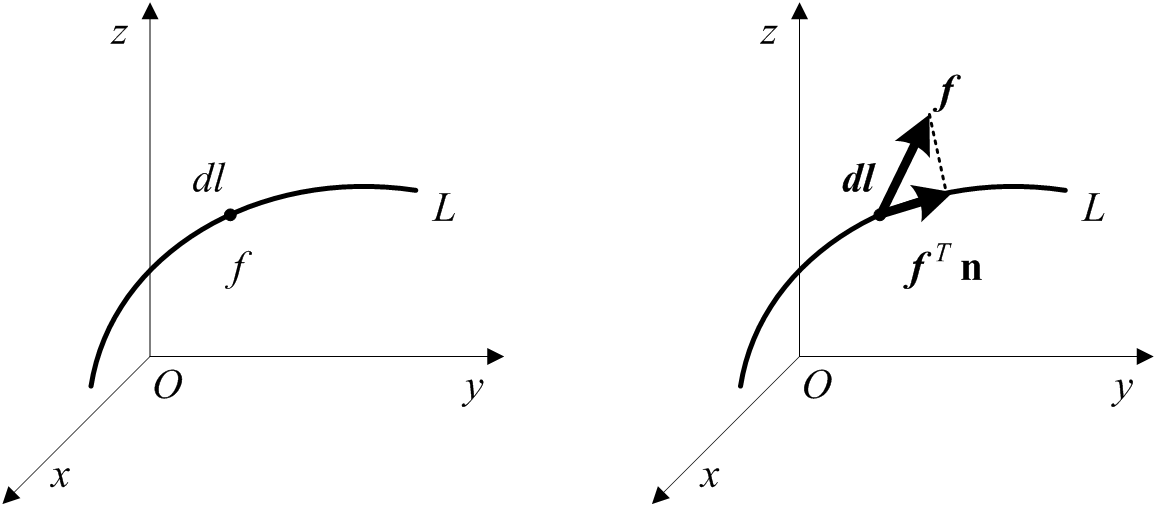
\includegraphics[height=3.5cm]{9.1.png}
\end{figure}

\begin{tcolorbox}
从式子上看,只要看到$dl$的,都是第一类曲线积分,有$dx,dy,dz$单独出现的,就是第二类曲线积分。
\end{tcolorbox}

%============================================================
\subsection{曲线积分的物理意义}

物理上,第一类曲线积分表示一个数量场对一段弧的积分,如绳的质量、非均匀带电曲线的电荷总量等。
第二类曲线积分是对一个矢量场进行环流积分,即求矢量场$\boldsymbol{f}\left( \boldsymbol{p} \right) $在沿某一环流$L$下的环流量。
如果矢量场是力场,则环流积分就是力沿该曲线作的功,如果矢量场是电场,则环流积分就是电势差。

%============================================================
\subsection{计算方法对比}

假设曲线
\[
L:\begin{cases}
	x=x\left( t \right)\\
	y=y\left( t \right)\\
	z=z\left( t \right)\\
\end{cases} \quad t\in \left[ t_1,t_2 \right]
\]
第一类曲线积分和第二类曲线积分:
\begin{align*}
&\begin{cases}
	\int_L{f\left( \boldsymbol{p} \right) dl}\\
	dl=\sqrt{\left( x' \right) ^2+\left( y' \right) ^2+\left( z' \right) ^2}\cdot dt\\
\end{cases} \\
&\Rightarrow \int\limits_L{f\left( \boldsymbol{p} \right) dl}=\int_{t_1}^{t_2}{\left[ f\left( t \right) \cdot \sqrt{\left( x' \right) ^2+\left( y' \right) ^2+\left( z' \right) ^2} \right] dt} \\
&\begin{cases}
	\int_L{\boldsymbol{f}\left( \boldsymbol{p} \right) ^T\boldsymbol{dl}}\\
	\boldsymbol{dl}=\mathbf{n}dl=\left( x'\,\,y'\,\,z' \right) ^Tdt\\
\end{cases} \\
&\Rightarrow \int\limits_L{\boldsymbol{f}\left( \boldsymbol{p} \right) ^T\boldsymbol{dl}}=\int_{t_1}^{t_2}{\left[ P\left( t \right) \cdot x'+Q\left( t \right) \cdot y'+R\left( t \right) \cdot z' \right] dt}
\end{align*}





\newpage
\section{习题}

\begin{exercise}
计算下列曲线积分,并指出是第一类曲线积分还是第二类曲线积分:
\begin{enumerate}
    \item $\int_L{xydx}$,其中$L:x^2+y^2=2x$,$\left( 0,0 \right) \rightarrow \left( 2,0 \right) $上半周。
    \item $\int_L{ydx+zdy+xdz}$,其中$
    L:\begin{cases}
        x^2+y^2=1\\
        x+z=1\\
    \end{cases}
    $,{\it x}轴从正向负看,逆时针一周。
    \item $\int_L{ydl}$,其中$L:\frac{x^2}{25}+\frac{y^2}{9}=1$,{\it x}轴上方部分。
\end{enumerate}
\end{exercise}

解:

1. 只对$dx$积分,即只对{\it x}轴进行积分,所以是第二类曲线积分,曲线$L$可以化为$\left( x-1 \right) ^2+y^2=1$,表示圆心为$\left( 1,0 \right) $、半径为1的圆,曲线化为参数方程求解:
\begin{align*}
&L:\begin{cases}
	x=1+\cos t\\
	y=\sin t\\
\end{cases} \quad t\in \left[ \pi ,0 \right] \\
&\int\limits_L{xydx}=\int_{\pi}^0{\left( 1+\cos t \right) \sin t\cdot d\left( 1+\cos t \right)}=\frac{\pi}{2}
\end{align*}

2. 分别对三个轴积分,所以是第二类曲线积分,曲线化为参数方程求解:
\begin{align*}
&L:\begin{cases}
	x=\cos t\\
	y=\sin t\\
	z=1-\cos t\\
\end{cases} \quad t\in \left[ 0,2\pi \right] \\
&\int\limits_L{ydx+zdy+xdz} \\
&=\int_0^{2\pi}{\sin t\left( -\sin t \right) dt+\left( 1-\cos t \right) \cos tdt+\cos t\sin tdt}=-2\pi
\end{align*}

3. 显然是第一类曲线积分,曲线化为参数方程求解:
\begin{align*}
&L:\begin{cases}
	x=5\cos t\\
	y=3\sin t\\
\end{cases} \quad t\in \left[ 0,\pi \right] \\
&\int\limits_L{ydl}=\int_0^{\pi}{\left[ 3\sin t\cdot \sqrt{\left( -5\sin t \right) ^2+\left( 3\cos t \right) ^2} \right] dt}=9+\frac{75}{4}\mathrm{arc}\sin \frac{4}{5}
\end{align*}

\begin{tcolorbox}
总体思路是将曲线换成参数方程,规划出参数的积分区间。
\end{tcolorbox}

~

\begin{exercise}
求螺旋线
\[
L:\begin{cases}
	x=R\cos t\\
	y=R\sin t\\
	z=kt\\
\end{cases}
\]
在区域$t\in \left[ 0,2\pi \right] $内的长度。
\end{exercise}

解:

这是典型的对弧长的积分,属于第一类曲线积分,可以认为$f\left( \boldsymbol{p} \right) \equiv 1$,于是:
\begin{align*}
\int\limits_L{f\left( \boldsymbol{p} \right) \cdot dl}&=\int_0^{2\pi}{\sqrt{\left( x' \right) ^2+\left( y' \right) ^2+\left( z' \right) ^2}dt} \\
&=\int_0^{2\pi}{\sqrt{\left( -R\sin t \right) ^2+\left( R\cos t \right) ^2+k^2}dt} \\
&=\int_0^{2\pi}{\sqrt{R^2+k^2}dt}=2\pi \sqrt{R^2+k^2}
\end{align*}

~

\begin{exercise}
平面上一半径为R的圆形细线,其中任一点处的线密度为该点到圆周某一固定直径距离的平方,求细线质量。
\end{exercise}

解:

根据题目得到线密度函数$\rho \left( \boldsymbol{p} \right) =y^2$,细线质量为线密度对弧长的积分,也即$\rho \left( \boldsymbol{p} \right) =y^2$在一整圈上的第一类曲线积分,我们只需要计算第一象限积分即可:
\begin{align*}
&M=4\int\limits_L{\rho \left( \boldsymbol{p} \right) \cdot dl}=4\int\limits_L{y^2\cdot dl}=4\int\limits_L{y^2\cdot \sqrt{\left( x' \right) ^2+\left( y' \right) ^2}\cdot dt} \\
&L=\left\{ \left( x,y \right) \middle| 0\leqslant x\leqslant 1,0\leqslant y\leqslant 1,x^2+y^2=1 \right\}
\end{align*}
将曲线转成参数方程求解:
\begin{align*}
&L:\begin{cases}
	x=R\cos t\\
	y=R\sin t\\
\end{cases} \quad t\in \left[ 0,\frac{\pi}{2} \right] \\
&\begin{aligned}
	M&=4\int\limits_L{y^2\cdot \sqrt{\left( x' \right) ^2+\left( y' \right) ^2}\cdot dt} \\
    &=4\int_0^{\frac{\pi}{2}}{R^2\sin ^2t\sqrt{\left( -R\sin t \right) ^2+\left( R\cos t \right) ^2}dt}\\
	&=4R^3\int_0^{\frac{\pi}{2}}{\sin ^2tdt}=2R^3\int_0^{\frac{\pi}{2}}{\left( 1-\cos 2t \right) dt}=\pi R^3\\
\end{aligned}
\end{align*}

~

\begin{exercise}
若向量值函数$\boldsymbol{f}\left( \boldsymbol{p} \right) =\left( y^2\,\,2xy \right) ^T$,计算沿抛物线$y=x^2$从$\left( 0,0 \right) $到$\left( 1,1 \right) $一段弧的曲线积分,若抛物线$y=\sqrt{x},\left( 0,0 \right) \rightarrow \left( 1,1 \right) $,重新计算曲线积分。
\end{exercise}

解:

很显然是第二类曲线积分:
\begin{align*}
&\int\limits_L{\boldsymbol{f}^T\boldsymbol{dl}}=\int_0^1{y^2dx+2xydy}=\int_0^1{\left[ x^4+2x\cdot x^2\cdot 2x \right] dx}=1 \\
&\int\limits_L{\boldsymbol{f}^T\boldsymbol{dl}}=\int_0^1{y^2dx+2xydy}=\int_0^1{\left[ x+2x\cdot \sqrt{x}\cdot \frac{1}{2\sqrt{x}} \right] dx}=1
\end{align*}

~

\begin{exercise}
设二维平面上有力场$\boldsymbol{F}$,方向指向原点,大小与该点到原点的距离成正比,若有质点沿椭圆$\frac{x^2}{a^2}+\frac{y^2}{b^2}=1$逆时针从$\left( a,0 \right) $运动到$\left( 0,b \right) $,求力场对质点作的功。
\end{exercise}

解:

很典型的第二类曲线积分,根据题意,可得力场和曲线:
\begin{align*}
&L:\begin{cases}
	x=a\cos t\\
	y=b\sin t\\
\end{cases} \quad t\in \left[ 0,\frac{\pi}{2} \right] \\
&\boldsymbol{F}\left( \boldsymbol{p} \right) =k\sqrt{x^2+y^2}\left( \begin{array}{c}
	-\frac{x}{\sqrt{x^2+y^2}}\\
	-\frac{y}{\sqrt{x^2+y^2}}\\
\end{array} \right) =\left( \begin{array}{c}
	-kx\\
	-ky\\
\end{array} \right)
\end{align*}
力场作功:
\begin{align*}
W&=\int\limits_L{\boldsymbol{f}\left( \boldsymbol{p} \right) ^T\boldsymbol{dl}}=\int\limits_L{Pdx+Qdy+Rdz}=\int\limits_L{\left( -kx \right) dx+\left( -ky \right) dy} \\
&=\int_0^{\frac{\pi}{2}}{\left[ \left( -ka\cos t \right) \left( -a\sin t \right) +\left( -kb\sin t \right) \left( b\cos t \right) \right] dt} \\
&=k\left( a^2-b^2 \right) \int_0^{\frac{\pi}{2}}{\sin t\cos tdt}=\frac{k}{2}\left( a^2-b^2 \right)
\end{align*}
质点从$\left( a,0 \right) $运动到$\left( 0,b \right) $过程中:
\begin{itemize}
    \item 当$a>b$时,质点在靠近圆心,力场做正功,$W>0$;
    \item 当$a<b$时,质点在远离圆心,力场做负功,$W<0$。
\end{itemize}

~

\begin{exercise}
设曲线
\[
L:\begin{cases}
	x=t\\
	y=t^2\\
	z=t^3\\
\end{cases} \quad t\in \left[ 0,1 \right]
\]
把第二类曲线积分$\int_L{Pdx+Qdy+Rdz}$化为第一类曲线积分。
\end{exercise}

解:

首先观察弧微分:
\begin{align*}
&\because \begin{cases}
	dx=dt\\
	dy=2tdt\\
	dz=3t^2dt\\
\end{cases} \\
&\therefore dl=\sqrt{\left( dx \right) ^2+\left( dy \right) ^2+\left( dz \right) ^2}=\sqrt{1+4t^2+9t^4}\cdot dt
\end{align*}
再看积分:
\begin{align*}
\int\limits_L{Pdx+Qdy+Rdz}&=\int\limits_L{Pdt+Q2tdt+R3t^2dt} \\
&=\int\limits_L{\left( P+Q2t+R3t^2 \right) \cdot dt} \\
&=\int\limits_L{\left( P+Q2t+R3t^2 \right) \cdot \frac{dl}{\sqrt{1+4t^2+9t^4}}} \\
&=\int\limits_L{\frac{P+2xQ+3yR}{\sqrt{1+4y+9y^2}}\cdot dl}
\end{align*}









